\section{Funkcja falowa}

\subsection{Eksperyment z dwoma szczelinami}
Eksperyment z dwoma szczelinami to doświadczenie, w którym światło przechodzi przez dwie szczeliny i na ekranie za nimi pojawia się interferencja.

\begin{figure}[H]
    \centering
    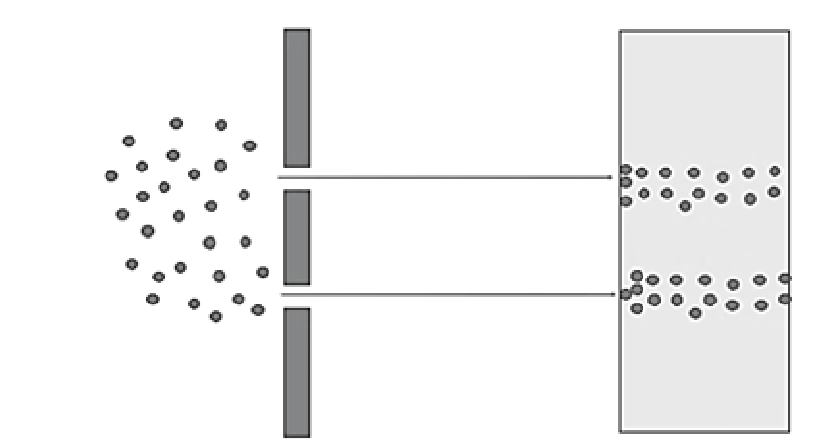
\includegraphics[width=0.5\textwidth]{szczeliny}
    \caption{Eksperyment z dwoma szczelinami. \textit{Źródło: Ranjbar, Vahid. (2023)}}
    \label{fig:szczeliny}
\end{figure}

\subsection{Eksperyment ze światłem}

\begin{figure}[H]
    \centering
    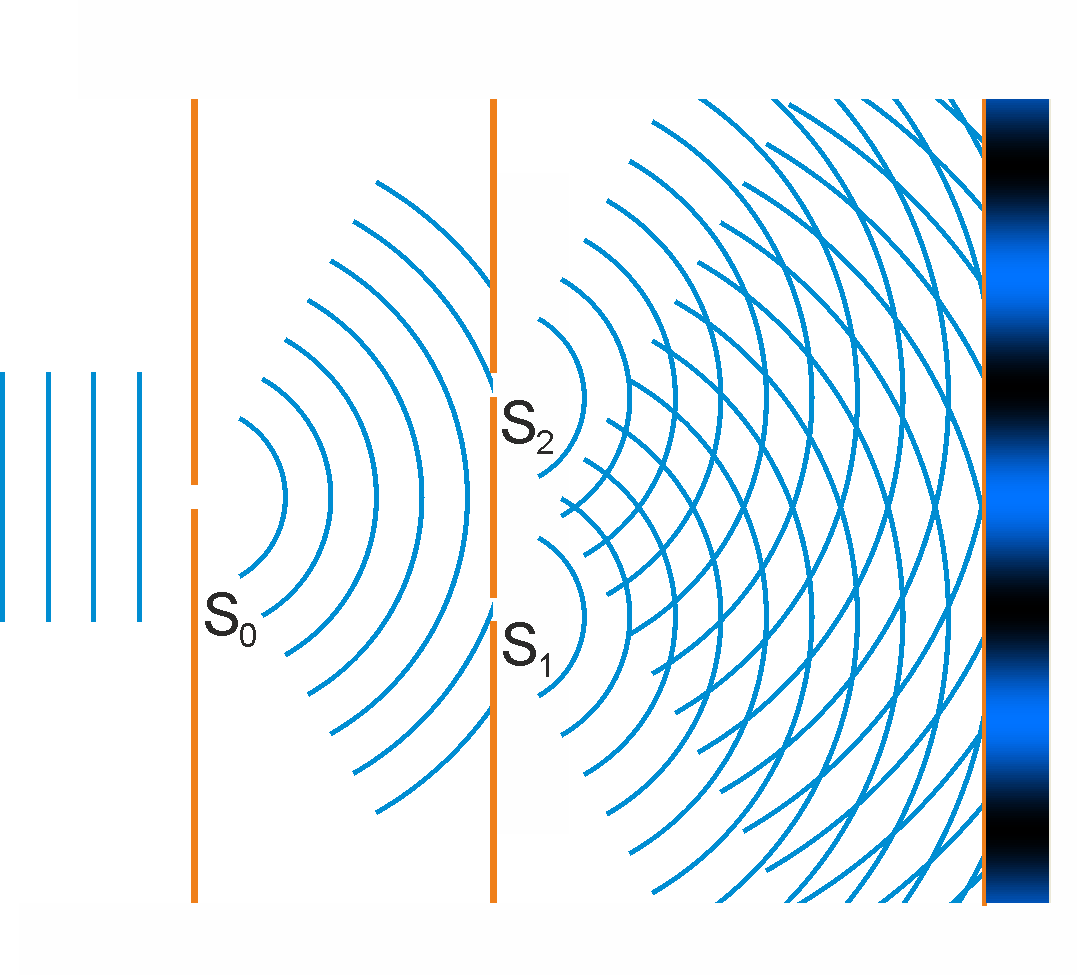
\includegraphics[width=0.5\textwidth]{szczeliny-fale}
    \caption{Eksperyment z dwoma szczelinami. \textit{Źródło: Zbigniew Kąkol, Jan Żukrowski (e-Fizyka, AGH)}}
    \label{fig:szczeliny-fale}
\end{figure}

Amplituda światła: $A(\vec{r}, t)$

Intensywność światła: $I = |A|^2$
\begin{equation*}
    I = |A_1|^2 + |A_2|^2 + A_1 A_2^* + A_1^* A_2
\end{equation*}
Jest to skutek superpozycji.

\subsection{Proste zagadnienie}

Amplitudy w dwóch miejscach:
\begin{equation*}
    A_1 = a_1 \exp[i(\omega t - k r_1 + \delta_1)]
\end{equation*}
\begin{equation*}
    A_2 = a_2 \exp[i(\omega t - k r_2 + \delta_2)]
\end{equation*}

Niech $a_1 = a_2 = a$ i $\delta_1 = \delta_2$. Dla dużych odległości ($D >> d$), fale są płaskie:
\begin{equation*}
    r_1^2 = D^2 + \left(x + \frac{d}{2} \right)^2
\end{equation*}
\begin{equation*}
    r_2^2 = D^2 + \left(x - \frac{d}{2} \right)^2
\end{equation*}

Stąd:
\begin{align*}
    r_1^2 - r_2^2 &= 2xd\\
    r_1 - r_2 &\approx \frac{xd}{D}
\end{align*}

Intensywność końcowa:
\begin{align*}
    I &= \left(a\cdot e^{i\omega t}\right)^2 \cdot \left[e^{-ikr_1}+e^{-ikr_2}\right] \\
    &= 2 a^2 \left(\cos{\left(kr_1-kr_2\right)}+1\right) \\
    &= 2 a^2 \left(1 + \cos{\left(k(r_1-r_2)\right)}\right) \\
    &= 2 a^2 \left(1 + \cos{\left(\frac{2\pi}{x}\cdot\frac{xd}{D}\right)}\right)
\end{align*}

\subsection{Funkcja falowa swobodnego elektronu}

$e^- \sim \text{fala}$ (formalna definicja później)

Niech $\Psi(x,y,z,t) \sim A(\vec{z}, t)$.  

$|\Psi|^2 = P$ -- ,,Intensywność'' fali elektronowej, prawdopodobieństwo znalezienia elektronu w tej chwili w danym miejscu.

Dla dwóch funkcji falowych:
\begin{equation*}
    \Psi = \Psi_A + \Psi_B
\end{equation*}
\begin{equation*}
    P \sim |\Psi_A + \Psi_B|^2
\end{equation*}

Prawdopodobieństwo znalezienia elektronu w danej przestrzeni $= 1$. Zatem
\begin{equation*}
    \int |\Psi(z,t)|^2 dz = 1.
\end{equation*}

Funkcja falowa znormalizowana do jedynki. Funkcja falowa jest całkowalna kwadratowo.

Superpozycja:
\begin{align*}
    \Psi &= c_1 \Psi_1 + c_2 \Psi_2 \\
    \Psi_1 &= |\Psi_1| e^{i \alpha_1} \\
    \Psi_2 &= |\Psi_2| e^{i \alpha_2}
\end{align*}
Stąd:
\begin{equation*}
    |\Psi|^2 = |c_1 \Psi_1|^2 + |c_2 \Psi_2|^2 + 2 \Re \left[ c_1 c_2 \Psi_1 \Psi_2 e^{i \alpha_1 - \alpha_2} \right]
\end{equation*}
